\subsubsection{Actividad 2 lab 3}
%*********************
%--------------------------------
\begin{frame}{Actvidad 3 lab 2}
\begin{figure}[H]
\begin{flushleft}
Objetivo:
\end{flushleft}
\begin{flushleft}
-Variar la  amplitud y fase de la señal para generar las curvas de Lissajous.
\end{flushleft}

\begin{center}
\centering
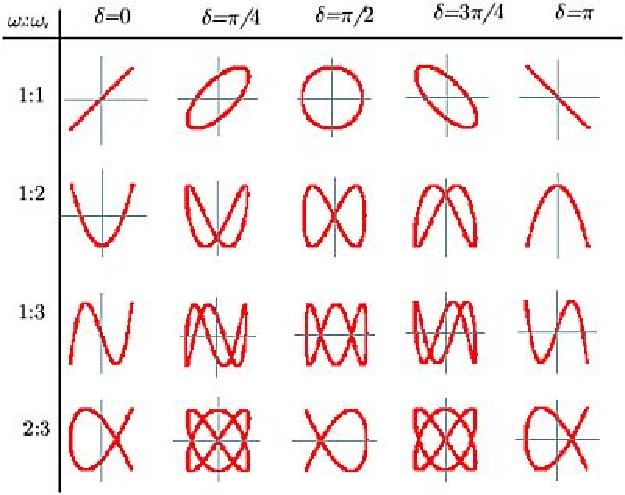
\includegraphics[width=0.65\textwidth]{parte1/lab2/pdf/lab2_19.pdf}
\end{center}
\end{figure}
\end{frame}
%--------------------------------
